\dev{Daphné Kany}{Balabonski MPI}

\textit{Dans cette leçon on présente le problème de la pyramide. C'est un exemple introductif à la programmation dynamique.}

\paragraph{Problème de la pyramide} \enspace\\ Entrée : Une pyramide $\Pi$ de hauteur h remplie d'entiers.\\ Sortie : La valeur maximale d'un chemin du sommet de la pyramide à sa base.

\begin{center}
	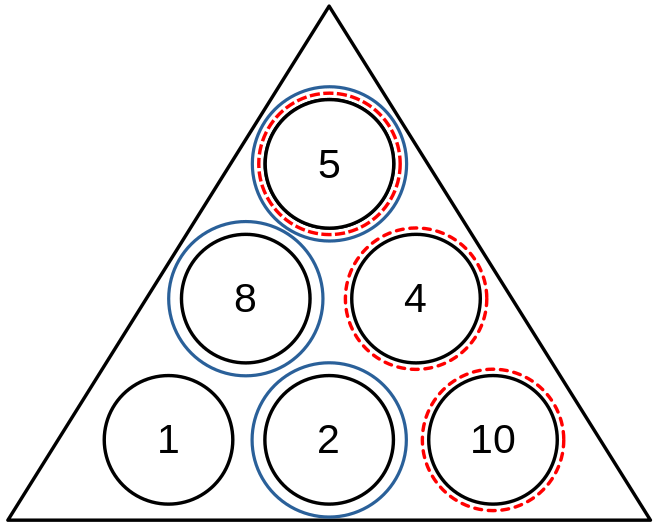
\includegraphics[scale=0.4]{Developpements/Pyramide/pyramide.png}
\end{center}

Exemple : pyramide de hauteur 3. En rouge, la valeur optimale d'un chemin depuis le sommet (19).

\begin{rem}
	Combien de chemins possibles ? $2^{h}$ \\
	Un algorithme exhaustif aura une complexité exponentielle.
\end{rem}

\paragraph{Approche gloutonne\\} A chaque étape, on choisit le sommet de plus grande valeur. Complexité : O(h).

\begin{com}
	Faire le glouton sur l'exemple au dessus. On trouve 15. Cela nous prouve que l'algorithme glouton n'est pas optimal. 
\end{com}

\begin{rem}
	L'algorithme glouton n'est pas optimal.
\end{rem}

\paragraph{Programmation dynamique}\enspace\\
Étape 1 (création des sous pb) : Si p est une sous pyramide de $\Pi$, on note S(p) la valeur max d'un chemin du sommet de p à sa base. \\
Étape 2 (relation de récurrence) : On note $\Pi_{g}$ et $\Pi_{d}$ les pyramides filles gauche et droite de $\Pi$. \\
\begin{center}$S(\Pi) = v(\Pi) + \max(S(\Pi_{g}), S(\Pi_{d}))$
\end{center}
où $v(\Pi)$ est la valeur du sommet de la pyramide.\\
Étape 3 : Implémentation

\paragraph{Représentation informatique de la pyramide}
\enspace\\
On va stocker notre pyramide dans un tableau T de dimension h*h. \\
T[i,j] = jème élément en partant de la gauche à la profondeur i si j $\leq$ i

$$ T : \: \begin{array}{|c|c|c|}
	\hline
	5 &  &  \\ \hline
	8 & 4 &  \\ \hline
	1 & 2 & 10 \\ \hline
\end{array}
$$

\begin{rem}
	Les sous pyramides gauches et droites de (i,j) sont (i+1, j) et (i+1, j+1)
\end{rem}

\paragraph{Méthode naïve sans mémoïsation} \enspace\\

\begin{algorithm}[H]
	\Entree{T le tableau représentant $\Pi$ ; 
	i et j les indices du sommet considéré}
	
	h = len(T) \\
	\Si{i == h} {
		retourner T[i,j]
	}
	\Sinon{
		retourner T[i,j] + max(cheminOpt(T, i+1, j), cheminOpt(i+1, j+1))
	}
	
	\caption{cheminOpt(T, i, j)}
\end{algorithm}

\begin{rem}
	Complexité : C(h) = 1 + 2C(h-1) donc C(h)=$2^{h}$. On retombe sur l'algorithme exhaustif qui énumère tous les chemins.
\end{rem}

\paragraph{Méthode descendante :} \enspace\\

\begin{com}
	Faire les modifications directement sur l'algo naïf au tableau
\end{com}

\begin{algorithm}[H]
	\Entree{T le tableau représentant $\Pi$ ; 
		i et j les indices du sommet considéré ; 
	R stocke les résultats intermédiaires}
	\Si{R[i,j] $>$ $- \infty$} {
		retourner R[i,j]
	}
	h = len(T) \\
	\Si{i == h} {
		R[i,j] = T[i,j] \\
		retourner R[i,j]
	}
	\Sinon{
		R[i,j] = T[i,j] + max(cheminOpt(T, i+1, j), cheminOpt(i+1, j+1)) \\
		retourner R[i,j]
	}
	
	\caption{cheminOpt(T, R, i, j)}
\end{algorithm}

\begin{rem}
	C(h) = h² car on remplit le tableau R une seule fois
\end{rem}

\paragraph{Méthode ascendante :} \enspace\\

\begin{algorithm}[H]
	\Entree{T le tableau représentant $\Pi$}
	h = len(T) \\
	R = tableau h*h \\
	\Pour{j allant de 1 à h} {
		R[h,j] = T[h,j]
	}
	\Pour{i de h-1 à 1}{
		\Pour{j de 1 à i}{
			R[i,j] = T[i,j] + max(R[i-1, j], R[1-1, j-1])
		}
	}
	retourner R[1,1]
	\caption{cheminOpt(T)}
\end{algorithm}

\begin{com}
	Dérouler la méthode ascendante sur l'exemple du début pour obtenir le tableau : 
\end{com} 

$$ T : \: \begin{array}{|c|c|c|}
	\hline
	19 &  &  \\ \hline
	10 & 14 &  \\ \hline
	1 & 2 & 10 \\ \hline
\end{array}
$$

\begin{com}
	S'il reste du temps : expliquer comment retrouver le chemin à l'aide d'un tableau prochainNoeud.
\end{com} 